\documentclass[a4paper]{article}

%% Language and font encodings
\usepackage[english]{babel}
\usepackage[utf8x]{inputenc}
\usepackage[T1]{fontenc}

%% Sets page size and margins
\usepackage[a4paper,top=3cm,bottom=2cm,left=3cm,right=3cm,marginparwidth=2cm]{geometry}

%% Useful packages
\usepackage{amsmath}
\usepackage{amsfonts}
\usepackage{bbm}
\usepackage{graphicx}
\usepackage[colorinlistoftodos]{todonotes}
\usepackage[colorlinks=true, allcolors=blue]{hyperref}
\usepackage{float}
\usepackage{enumerate}
\usepackage{mathrsfs}
\usepackage{subcaption}

\usepackage{tikz}
\tikzset{
    vertex/.style={circle,draw,minimum size=1.5em},
    edge/.style={->,> = latex'}
}

\title{Stochastic Processes}
\author{Kevin Chang}

\graphicspath{ {./images/} }

\begin{document}
\maketitle

\section{1.2}
\begin{itemize}
    \item (a)
        \begin{itemize}
            \item $\mathit{Range}(F(X)) := [0, 1]$
            \item For $x \in [0, 1]$
                \begin{itemize}
                    \item $P[F(X) \leq x] = P[X \leq F^{-1}(x)] = F(F^{-1}(x)) = x$
                \end{itemize}
            \item For $x > 1$
                \begin{itemize}
                    \item $P[F(X) \leq x] = P[F(X) \leq 1] = 1$
                \end{itemize}
            \item For $x < 0$
                \begin{itemize}
                    \item $P[F(X) \leq x] = P[F(X) < 0] = 0$
                \end{itemize}
        \end{itemize}
    \item (b)
        \begin{itemize}
            \item $\mathit{Range}(F(X)) := [0, 1]$
            \item $P[F^{-1}(U) \leq x] = P[U \leq F(x)] = F(x)$
        \end{itemize}
\end{itemize}

\section{1.3}
\begin{itemize}
    \item $P[X_n = i] = \binom{n}{i} p_n^k (1 - p_n)^{n-k}$
    \item $P[X_n = i] = \lim_{n\rightarrow \infty} \binom{n}{i}(p_n)^i(1 - p_n)^{n-i}$

    $= \lim_{n\rightarrow \infty} \binom{n}{i}(\frac{\lambda}{n})^i(\frac{n-\lambda}{n})^{n-i}$

    $= \frac{\lambda^i}{i!}\lim_{n\rightarrow \infty} \frac{n! \times n^{i}}{(n-i)! n^i (n-\lambda)^i} (\frac{n-\lambda}{n})^n$

    $= \frac{\lambda^i}{i!}(1-\frac{\lambda}{n})^{n} = \frac{\lambda^i}{i!}\exp(-\lambda)$
\end{itemize}

\section{1.35}
\begin{itemize}
    \item (a)
        \begin{itemize}
            \item $\mathbb{E}[h(X)] = \int_{-\infty}^\infty h(x) f(x) dx = \int_{-\infty}^\infty h(x) e^{-tx} M(t) f_t(x)dx = \mathbb{E}[e^{-tX_t}h(X_t)] M(t)$
        \end{itemize}
    \item (b)
        \begin{itemize}
            \item $P[X > a] = \int_a^\infty f(x) dx = \int_a^\infty e^{-tx} M(t) f_t(x) dx \leq \int_a^\infty e^{-ta} M(t) f_t(x) dx$

                $= M(t) e^{-ta} P[X_t > a]$
        \end{itemize}
    \item (c)
        \begin{itemize}
            \item 
        \end{itemize}
\end{itemize}

\section{1.36}
\begin{itemize}
    \item Jensen's Inequality
        \begin{itemize}
            \item $f(\sum_i w_i x_i) \leq \sum_i w_i f(x_i)$ with non-negative $w_i$ summing to 1
        \end{itemize}
    \item choose $f(x) = -\log x$ and $w_i = \frac{1}{n}$

        $\rightarrow -\log(\frac{1}{n} \sum_i x_i) \leq - \frac{1}{n} \sum_i \log x_i$
    \item inverse the equation and apply exponential on both side

        $\rightarrow \frac{1}{n} \sum_i x_i \geq (\prod_i x_i)^{\frac{1}{n}}$
\end{itemize}

\section{Computer Problem}

\begin{figure} [b]
	\centering
	\begin{subfigure}[t]{0.45\textwidth}
        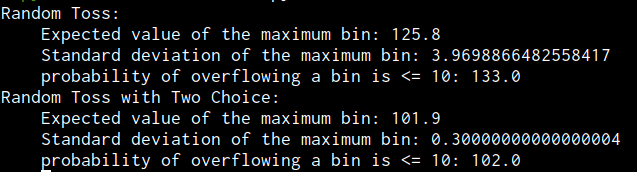
\includegraphics[width=\linewidth]{src/result.png}
      \caption{Result of the simulation}
    \end{subfigure}
    ~
    \begin{subfigure}[t]{0.45\textwidth}
        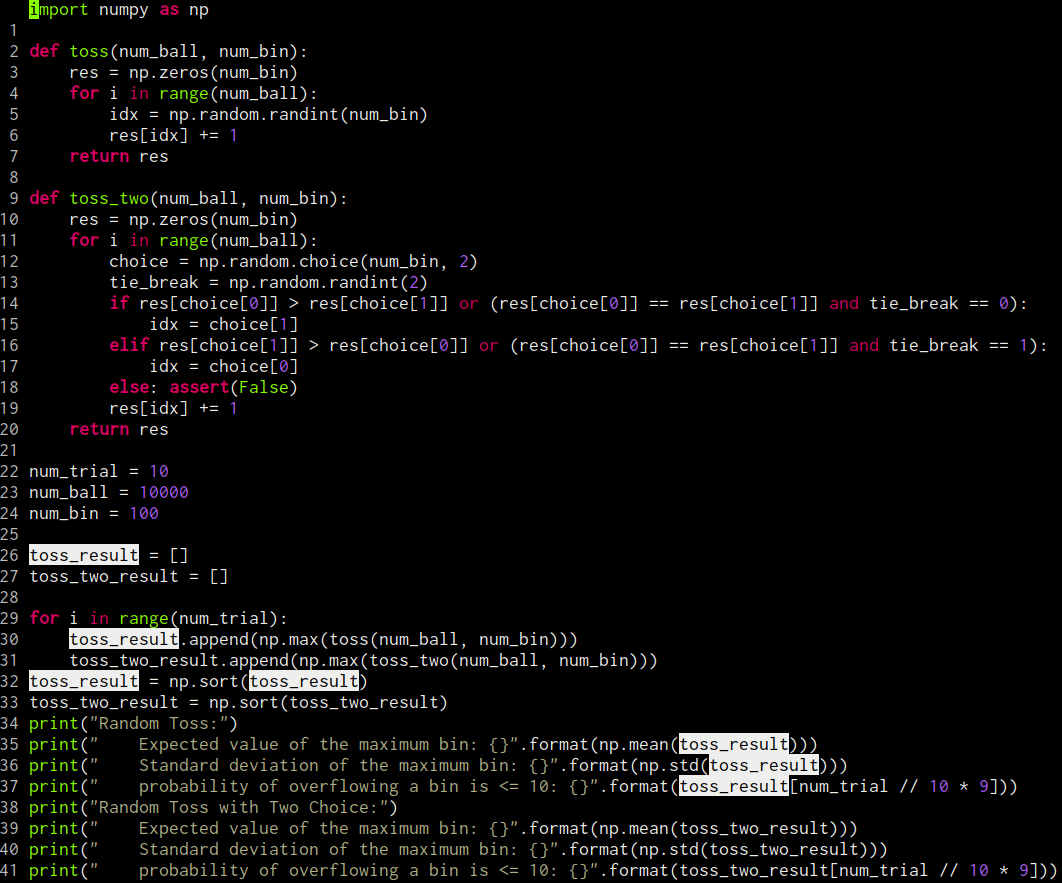
\includegraphics[width=\linewidth]{src/code.png}
        \caption{Code}
    \end{subfigure}
\end{figure} 

\end{document}
